\documentclass{article}

\usepackage{graphicx}
\usepackage{tikz}
\usepackage{tikzsymbols}
\usetikzlibrary{calc,patterns,shapes.geometric}
\pagestyle{empty}
\usepackage[margin=0pt]{geometry}
\geometry{papersize={14in,12in}}

\def\centerarc[#1](#2)(#3:#4:#5){\draw[#1] ($(#2)+({#5*cos(#3)},{#5*sin(#3)})$) arc (#3:#4:#5);}

\begin{document}
	\begin{figure}
		\centering
		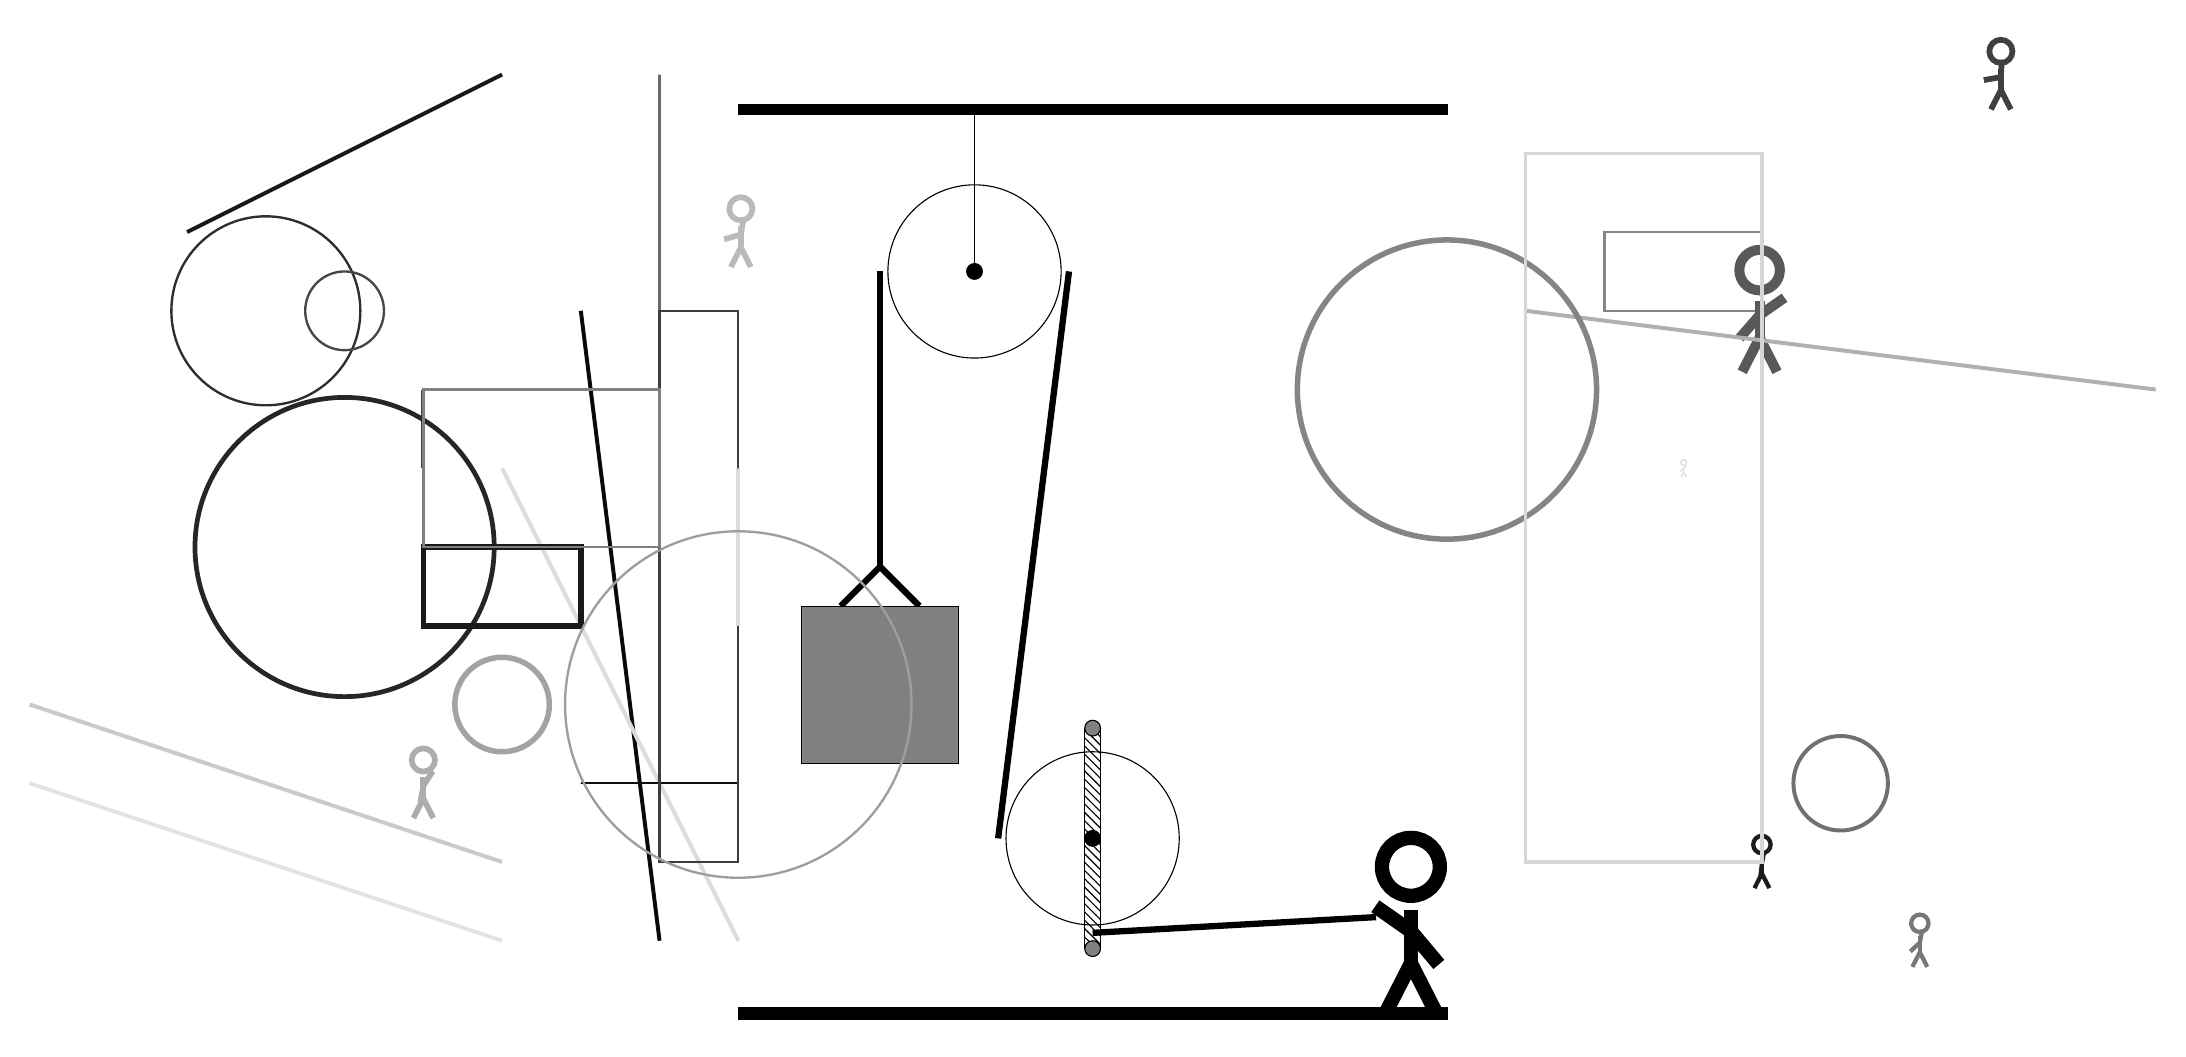
\begin{tikzpicture}
			%%%%% START %%%%%
			
			\draw[fill=black] (-2, 11.5) rectangle (7, 11.625);
			
			\draw (1, 9.5) circle (1.1);
			\draw[fill=black] (1, 9.5) circle (0.1);
			\draw (1, 11.5) -- (1, 9.5);
			
			\draw[fill=white](2.5, 2.3) circle (1.1);
			\draw[fill=black] (2.5, 2.3) circle (0.1);
			\draw[pattern=north west lines, pattern color=black] (2.4, 3.7) rectangle (2.6, 0.9);
			\draw[fill=black!50] (2.5, 3.7) circle (0.1);
			\draw[fill=black!50] (2.5, 0.9) circle (0.1);
			
			\draw[line width=0.8mm] (-0.7, 5.25) -- (-0.2, 5.75) -- (0.3, 5.25);
			\draw[fill=black!50] (-1.2, 5.25) rectangle (0.8, 3.25);
			
			\draw[line width=0.8mm] (-0.2, 9.5) -- (-0.2, 5.75);
			\centerarc[line width=0.8mm](1, 9.5)(0:180:1.2000000000000002);
			\draw[line width=0.8mm](2.2, 9.5) -- (1.3, 2.3);
			\centerarc[line width=0.8mm](2.5, 2.3)(180:270:1.2000000000000002);
			\draw[line width=0.8mm](2.5, 1.1) -- (6.1, 1.3);
			
			\node at (6.5, 1.2) {\Strichmaxerl[10][-35][-50]};
			
			\draw[line width=0.5mm, color=black!96](-4, 9) -- (-3, 1);
			
			\draw[line width=0.5mm, color=black!14](-5, 7) -- (-2, 1);
			\draw[line width=0.5mm, color=black!11](-5, 1) -- (-11, 3);
			\node[line width=0.7mm, color=black!53] at (13, 1) {\Strichmaxerl[3][43][79]};
			
			\draw[line width=0.3mm, color=black!59] (-3, 12) rectangle (-3, 4);
			\draw[line width=0.5mm, color=black!21](-5, 2) -- (-11, 4);
			\draw [line width=0.5mm, color=black!56](12, 3) circle (0.6);
			\draw[line width=0.5mm, color=black!75](-6, 8) -- (-6, 7);
			\node[line width=0.3mm, color=black!27] at (-2, 10) {\Strichmaxerl[4][16][80]};
			\node[line width=0.4mm, color=black!75] at (14, 12) {\Strichmaxerl[4][10][87]};
			\draw [line width=0.6mm, color=black!85](-7, 6) circle (1.9);
			\draw [line width=0.3mm, color=black!82](-8, 9) circle (1.2);
			\draw [line width=0.7mm, color=black!36](-5, 4) circle (0.6);
			\draw[line width=0.3mm, color=black!48] (9, 9) rectangle (11, 10);
			\node[line width=0.7mm, color=black!13] at (10, 7) {\Strichmaxerl[1][30][51]};
			\draw[line width=0.3mm, color=black!95] (-2, 3) rectangle (-4, 3);
			\draw[line width=0.7mm, color=black!90] (-4, 6) rectangle (-6, 5);
			
			\node[line width=0.5mm, color=black!89] at (11, 2) {\Strichmaxerl[3][83][80]};
			\node[line width=0.4mm, color=black!32] at (-6, 3) {\Strichmaxerl[4][80][57]};
			\draw[line width=0.3mm, color=black!76] (-3, 9) rectangle (-2, 2);
			\node[line width=0.5mm, color=black!65] at (11, 9) {\Strichmaxerl[7][49][35]};
			
			\draw[line width=0.5mm, color=black!31](8, 9) -- (16, 8);
			
			\draw[line width=0.5mm, color=black!14] (-2, 5) rectangle (-2, 7);
			\draw [line width=0.7mm, color=black!48](7, 8) circle (1.9);
			\draw[line width=0.4mm, color=black!16] (8, 11) rectangle (11, 2);
			
			\draw [line width=0.3mm, color=black!72](-7, 9) circle (0.5);
			\draw[line width=0.5mm, color=black!90](-5, 12) -- (-9, 10);
			\draw [line width=0.6mm, color=black!40](-5, 10) circle (0.0);
			\draw[line width=0.3mm, color=black!50] (-3, 8) rectangle (-6, 6);
			
			\draw [line width=0.3mm, color=black!38](-2, 4) circle (2.2);
			
			\draw[fill=black] (-2, 0) rectangle (7, 0.15);
			
			%%%%% END %%%%%
		\end{tikzpicture}
	\end{figure}	
\end{document}